% !TEX root = ../thesis.tex
% !TEX root = single_chapter_intro.tex
\chapter{Introduction}
\label{chap:intro}

For millennia mankind has watched and studied the night sky. Apart from planets and comets it appeared as an immutable canvas on which the stars rested. It comes as no surprise that for ancient civilisations supernovae (which were very rare events, occurring only every few centuries ) were interpreted as important omens as they broke the paradigm of the unchanging night skies. As these events are so rare their origin remained a mystery until in the first half of the last century. \citet{1934PNAS...20..254B} suggested that \textit{``the phenomenon of a super-nova represents the transition of an ordinary star into a body of considerably smaller mass''}. For the last 85 years the supernova-branch of astronomy has been developing. There have been many advances, but there are still many unknowns. This thesis addresses two sub fields of supernovae: The unsolved progenitor problem for Type Ia supernovae as well as quantifying the nucleosynthetic yield and energies of Type Ia supernovae.


\section{Ancient Supernovae}
\label{sec:ancientsn}
Although supernovae must have been observed since the beginning of humankind, reliable records only exist for the last thousand years. There are however transient star sightings mentioned in older text. For example, \textit{Houhanshu} \citep{2006ChJAA...6..635Z}, mentions a new star which was visible for 8 months (depending on the interpretation of the text it could also mean 20 months) in the year of AD185. This new star was reported to be in the \textit{Nanmen} asterism which is close to \gls{alphacen}.  Observations in modern times have revealed a supernova remnant in a distance of roughly 1~\kpc\ near \gls{alphacen} \citep{2006ChJAA...6..635Z}. Some believe this to be evidence that the star mentioned in the ancient text is  the oldest written record of a supernova, others however interpret this text as reference to a comet \citep{1994Natur.371..398C}. 

The oldest undisputed record of a supernova is \sn{1006}{}, which also coincides with the brightest ever recorded supernova.  It was observed worldwide by Asian, Arabic and European astronomers. \citet{1965AJ.....70..105G} gives a good summary of the observations and interpretation given by these ancient observers. Ali Ibn Ridwan was an Egyptian astronomer who recorded the appearance of \sn{1006}{}. He wrote in a comment on Ptolemy's Tetrabiblos: 
\begin{quote}
\textit{``I will now describe for you a spectacle that I saw at the beginning of my education. This spectacle appeared in the zodiacal sign Scorpio in opposition to the sun, at which time the sun was in the 15th degree of Taurus, and the spectacle in the 15th degree of Scorpio. It was a large spectacle, round in shape and its size 2.5 or 3 times the magnitude of Venus. Its light illuminated the horizon and twinkled very much. $\dots$ This apparition was also observed at the time by (other) scholars just as I have recorded it.''}
\end{quote}

Only 50 years after the bright supernova of 1006, Chinese and Japanese astronomers reported on another cataclysmic event which was at first even visible during the day.  \sn{1054}{} might have also been observed in North America where petroglyphs in the Chaco Canyon could be interpreted as a depiction of this event (see Figure \ref{fig:sn1006_chaco}). It is difficult to date  these cave paintings precisely, but they were created around the time of the \sn{1054}{} explosion. It is still debated if \sn{1054}{}\ was the inspiration of the painting or the inspiration came from the passing of Hailey's comet in 1066. More than 900 years later \citet{1968Sci...162.1481S} detected a pulsar in the centre of \sn{1054}{}. This was the first time that the stellar remnant connected with a known supernova was found.
\sn{1181}{} ends the 180 year period with three confirmed supernovae that started with \sn{1006}. This Galactic supernovae  first discovered in August of 1181 was visible for about half a year and was mentioned in eight different texts by Chinese and Japanese astronomers. 3C58, a pulsar found in \sn{1181}{}, is suggested to be the neutron star remnant of this stellar explosion. 



\begin{figure}[tb] %  figure placement: here, top, bottom, or pag
   \centering
   \includegraphics[width=\textwidth]{chapter_intro/plots/Chaco_canyon_pueblo_bonito_petroglyphs.jpg} 
   \caption[Chaco canyon petroglyphs]{Chaco canyon petroglyphs show a hand, a moon and a bright celestial object. This could be SN1054 but it is ambiguous. (Source Wikipedia/ Photographer jamesdale10/ Creative Commons license)}
   \label{fig:sn1006_chaco}
\end{figure}

Humanity had to wait for nearly 400 years before the next bright event occurred. Although the supernova was discovered by an abbot in Messina on 06 November 1572, Tycho Brahe is often attributed the discovery of this event. The attribution of \sn{1572}{} to Tycho came from his angular distance and brightness measurements of unprecedented precision (location to a few arc minutes!; see Figure \ref{fig:sn1572_tycho_chart}). These precise measurements proved that the star changed in brightness but stayed at a fixed position like stars. Therefore Tycho concluded that this transient event was far beyond the moon, where stars were suspected to be located. This broke the paradigm of the constancy of stars, which was believed by many. Having been studied for almost one and a half years the supernova finally faded from visibility in March 1574. The measurements of \sn{1572}{}, among other astronomy related subjects, were published by \cite{1602QB41.B73.......}. Another 400 years elapsed before radio emissions identified the remains of \sn{1572}{} \citep{1952Natur.170..364H}.


\begin{figure}[tb] %  figure placement: here, top, bottom, or page
   \centering
   \includegraphics[width=0.7\textwidth]{chapter_intro/plots/Tycho_Cas_SN1572.jpg} 
   \caption[Star chart of SN 1572 by Tycho Brahe]{Brahe, Tychonis [A facsimile reprint of the original edition, 1573]. The supernova is marked with the letter I. The caption reads: \textit{``I have indeed measured the distance of this star from some of the fixed stars in the constellation of Cassiopeia several times with an exquisite (optical) instrument, which is capable of all the fine details of measurement. I have further detected that it (the new star) is located 7 degrees and 55 minutes from the star at the breast of the Schedir designated by B.''} translation kindly provided by Leonhard Kretzenbacher}
   \label{fig:sn1572_tycho_chart}
\end{figure}

Kepler, working with Tycho, discovered \sn{1604}{} nearly 20 days before maximum light, which occurred on the 28th of October 1604. Serendipitously, around this time there was a conjunction of Jupiter and Mars, which was observed by many astronomers. This also led to an early upper limit, where astronomers described the conjunction but did not mention the supernova. As Tycho did before him, Kepler measured the location and the brightness of the supernova precisely \citep[see Figure \ref{fig:sn1604_ancient_lc};][]{kepler1606} before it faded from visibility 18 months later. Kepler was not the only astronomer observing \sn{1604}\ and there exist many texts from Korea and China mentioning this event. \sn{1604}{} was the last confirmed observation of a supernova in our own Galaxy. A good review of these ancient supernovae can be found in \citet{2003LNP...598....7G}.

Observations in modern times have revealed two additional supernovae that must have exploded after \sn{1604}\ but are not mentioned in the historical literature. \gls{casa}, a supernova remnant, is the brightest radio source in the sky. It has been estimated that this supernova should have been visible between 1660 and 1680, however there are no clear descriptions or references from astronomers in the seventeenth century. There has been much speculation to the reason (e.g. heavily obscured by interstellar dust and thus not visible), but it still remains unclear why it was not observed. \citet{1984Natur.312..527G} detected another supernova remnant right in the heart of our Galaxy. Recent \xray\ observations revealed the supernova to be less than 150 years old \citep{2008ApJ...680L..41R}. This supernova happened very close to the galactic centre and is heavily obscured by dust. At the time of explosion it was not visible at optical wavelengths. 
\begin{figure}[tb] %  figure placement: here, top, bottom, or page
   \centering
   \includegraphics[width=\textwidth]{chapter_intro/plots/sn1604_ancient_lc.pdf} 
   \caption[Light curve of SN 1604]{Light curve of \sn{1604}{}\ obtained by ancient European and Korean astronomers. There is a European upper limit on the 8th of October 1604. Comparing these 400 year old measurements with modern day light curve templates by \citet{2011MNRAS.412.1441L} show clearly that the supernova is a Type Ia supernova. Historical data graciously supplied by D.A. Green \citep{1977QB841.C58......, 2003LNP...598....7G}}
   \label{fig:sn1604_ancient_lc}
\end{figure}
In summary, the five ancient supernovae (\sn{1006}{}, \sn{1054}{}, \sn{1181}{}, \sn{1572}{} and \sn{1604}{}) were all observed without the use of a telescope. Our ancient astronomy colleagues had only very primitive means to observe supernovae. However, the remarkably precise written records can be attributed to their ingenuity and assiduity. Even in an era of 10-meter telescopes the records of these explosions remain useful (see Figure~\ref{fig:sn1604_ancient_lc}).




\section{Modern Supernova Observations and Surveys}
\label{sec:surveys}

The era of modern supernova observations started with the discovery of \sn{1885}{}. \sn{1885}{} (also known as S Andromedae) was first spotted by Isaac Ward in Belfast in August of 1885 \citep{1885AN....112..360H} and was visible until February 1886. 
More than 50 years later \citet{1934PNAS...20..254B} coined the term supernova and established the difference between common novae and supernovae. \citet{1934PNAS...20..254B} also suggested that these luminous events are caused by the deaths of stars. 

In order to understand the phenomenon of supernovae better, Zwicky began a supernova search with the 18-inch Schmidt telescope. In those days the detectors were photographic plates, which were analysed with the help of a blink comparator. This device permitted rapid switching between viewing two different photographic plates which were observed on different nights and one could easily detect \textit{new stars}. Using this method Zwicky found several supernovae which in turn inspired Minkowski to classify these supernovae by their spectra \citep{1941PASP...53..224M}. 
Minkowski categorised the 14 known objects into two categories. Those without hydrogen he called \emph{Type I}, those with hydrogen he called \emph{Type II} (see Section~\ref{sec:sn_classification} for a more detailed description of supernova classification).

With the advent of computing in the 1960s the first computer-controlled telescopes were built. A 24-inch telescope was constructed by the Northwestern University and deployed at the Corralitos Observatory in New Mexico with the express purpose of undertaking a \gls{dass}. While ultimately unsuccessful in finding supernovae, this search lead the way in computer controlled discovery and many later surveys would employ a similar design.

The advancements of detector technologies in 1980s, such as photoelectric photometers and later \glspl{ccd}, together with increasing power and connectivity of computers, enabled the construction of automated telescopes with minimal human interaction \citep[e.g.][]{1986IAUS..118...47G}. These first automated telescopes were used mainly for variable star surveys. 

The \gls{bait} was one of the first automated telescopes designed specifically to find supernovae. This search produced 15 supernova discoveries by 1994 \citep{1994AAS...185.7905V}, including the famous \sn{1994}{D}, pictured here (Figure \ref{fig:sn1994d}). Due to increasing light pollution in Berkley this project moved to the Lick Observatories and was named the \gls{loss}. With the switch to the new observatory the \gls{bait} was replaced with the \gls{kait}. \gls{loss} has been one of the most successful supernova surveys to date. By the year 2000 it had found 96 supernovae \citep{2001ASPC..246..121F}. 

\begin{figure}[tb] %  figure placement: here, top, bottom, or page
   \centering
   \includegraphics[width=\textwidth, trim=4cm 4cm 4cm 10cm, clip=true, keepaspectratio]{chapter_intro/plots/sn1994d.jpg} 
   \caption[HST image of SN 1994D]{\sn{1994}{D} in \object{NGC 4526} taken with the same \glsentryname{hst}. This image shows very clearly how the light from the explosion of only one star can outshine an entire galaxy (Pete Challis/NASA). This picture is also widely used in popular astronomy.}
   \label{fig:sn1994d}
\end{figure}

In the mid to late 1990s, as high quality data on supernovae became available (mainly contributed by the \gls{ctss}), the long dream \citep[e.g.][]{1938ApJ....88..285B, 1960ZA.....49..201V, 1968AJ.....73.1021K} of using these objects as reliable distance indicators finally became viable. Two main teams drove the advancement in the cosmological distance measurements (the \gls{scp} and the \gls{hzsns}) and independently arrived at the same conclusion: the expansion of the universe is accelerating \citep{1998AJ....116.1009R,1999ApJ...517..565P}. For a more detailed overview of supernova cosmology see Section~\ref{sec:intro:sncosmology}.

By the turn of the millennium and following the discovery of the accelerated expansion of the universe, a variety of groups started large surveys specifically for supernovae. Among them were the \gls{essence} project and \gls{snls}. Both these programs have finished taking data, but have yet to publish all of their observations. Specialised surveys like the Nearby Supernova Factory \citep{2002SPIE.4836...61A} used an \gls{ifu} to capture light curves and spectra at the same time. The Higher-z survey \citep{2004ApJ...613..200S} focused on a high redshift range, available only through the \gls{hst}.

This effort is continued by a multitude of large sky surveys that have started in recent years (or are just about to). Some of these focus exclusively on transients and supernovae, like the \gls{ptf}, whereas others, like the \gls{panstarrs} and \gls{skymapper}, have transient/supernova components. Upcoming surveys, like the \gls{lsst} and the space-based \gls{gaia} mission, will provide unprecedented detail about current supernova types as well finding several new classes of transients \citep[e.g. \gls{gaia} will find $\approx14,000$ \sneia\ during its mission lifetime;][]{2003MNRAS.341..569B}.

In addition to supernova searches in the optical, searches have commenced at other wavelengths and other physical messengers. \glspl{grb} were first detected, as the name suggests, in \gammaray s and are thought to be the bolometrically brightest  transients. The first detection of a \gls{grb} was on July 2 of 1967 by a Vela satellite. Vela satellites where designed to monitor \gammaray\ signatures of banned nuclear weapons testing. It became quickly clear, due to the unusual form and direction of the signal, that these new \glspl{grb} where not of terrestrial origin. Six years later, the results from the Vela satellites were declassified and the existence of these \glspl{grb} made known to the world \citep{1973ApJ...182L..85K}. 

%Following on from the discovery of \glspl{grb} in 1973, 1000s of GRBs were observed by BATSE. A direct connection to SN was made via Beppo-Sax 9 as decribed via 98bw (underluminous), HETE-2 through 2003dh (normal brightness). This work continues with the SWIFT mission. 

At the beginning of the 1990s, new high-energy instruments like the \gls{batse} surveyed the sky in \gammaray s and detected thousands of \glspl{grb}. \citet{1992Natur.355..143M} showed that \glspl{grb}, due to their isotropic distribution, are events at cosmological distances rather than coming from our own Galaxy. The \gls{bepposax} satellite, launched in 1996, was able to provide accurate positions for \glspl{grb}. This advancement led to the discovery that \glspl{grb} occur in distant galaxies, establishing them as one of the most luminous events in the universe ($>10^{52}$~erg). The co-location of \sn{1998}{bw} and \grb{980425} established the connection between supernovae and some \glspl{grb} \citep{1998Natur.395..670G}. A class of short \glspl{grb} has remained supernovaless  \citep[e.g.]{2009ApJ...696..971X}. The subsequent \gls{hete2} mission established a new class of transients called \xray-flashes. These new objects are thought to be similar to  \glspl{grb} in physical nature but much less energetic \citep{2004ApJ...601L.119Z}. Such work continues with the \gls{swift} mission. 

Astronomy has been largely based on \EM\ waves, but there are other messengers of astrophysical information. Gravitational waves, predicted by the theory of general relativity  \citep{1918SPAW.......154E}, might provide us with another insight into supernovae. The most advanced detector today, the \gls{ligo} has not yet detected gravitational waves, although modelling indicates that it would have been highly unlikely, to have an event close enough to have been detected by \gls{ligo}. \gls{aligo} will likely detect gravitational waves from in-spiralling neutron stars, and possibly core collapse supernovae. The \gls{lisa}, an ambitious mission planned for the coming decade, is definitely sensitive enough to detect the predicted gravitational waves (a non-detection would show problems with the theory of general relativity). In the supernova field \gls{lisa} might give us an estimate on the number of in-spiralling white dwarfs, which are suggested as progenitors of \sneia.

\sn{1987}{A} was the first and only occasion on which neutrino emission from a supernova has been measured \citep{1987PhRvL..58.1494B,1987PhRvL..58.1490H,Alekseev:1988gp}. New, more sensitive detectors, like IceCube \citep{2008ICRC....4..835K}, will hopefully enable accurate neutrino observations of future Galactic supernovae.

For now, the optical observations of supernovae provide the bulk of observations of these transients. Hopefully, future instruments and capabilities will enable us to combine measurements across the \EM\ spectrum with gravitational wave and particle flux observations. Such an approach will unlock many of the secrets still held by these mysterious objects.

\section{Observational Properties of Supernovae}

\subsection{Supernova classification}
\label{sec:sn_classification}

The classification of supernovae started in 1941 when Minkowski realised that there seem to be two main types \citep{1941PASP...53..224M}. Those containing a \gls{halpha} line he called Type II supernovae and those showing no hydrogen he called Type I supernovae. This basic classification has remained to this day, however the two main classes branched into several subclasses. During the 1980s, the community discovered that most \sneia\ showed a broad \ion{Si}{2} line at 6130~\AA. There was, however, a distinct subclass of objects that lacked this feature. These silicon-less objects were then subclassed further into objects that showed helium -- now known as \gls{snib} --  and those that did not, called \gls{snic} \citep[see spectra in Figure \ref{fig:sn_classification};][]{1987ApJ...317..355H, 1986ApJ...306L..77G}. The classical Type I supernova was renamed to \snia. Today we know that \sneia\ originate from the explosion of white dwarfs. \sneii\ and \sneibc\ are believed to stem from the collapsing core of a massive star. 

\begin{figure}[tb] %  figure placement: here, top, bottom, or page
   \centering
   \includegraphics[width=\textwidth]{chapter_intro/plots/sn_classification.pdf} 
   \caption{Classification scheme by \citet{2003LNP...598...21T}}
   \label{fig:sn_classification}
\end{figure}

\begin{figure}[tb] %  figure placement: here, top, bottom, or page
   \centering
   \includegraphics[width=\textwidth]{chapter_intro/plots/sn_class_spectra.pdf} 
   \caption{Spectral comparison from \citet{2003LNP...598...21T}}
   \label{fig:sn_class_spectra}
\end{figure}

Only in the past two decades have we been able to explore the finer details of the \sneia\ class. Most objects have a small brightness scatter and are referred to as \gls{branchnormal}. In this class of \gls{branchnormal} \sneia, the community has found additional features that vary with brightness. For example, \citet{2005ApJ...623.1011B} found that the evolution of the \gls{vph} measured from the Doppler shift of the \ion{Si}{2} line at 6355~\AA\ is faster in more luminous \sneia\ (high velocity gradient - HVG)\glsadd{hvg} and slower in fainter \sneia\ (low velocity gradient - LVG) \glsadd{lvg}. Additionally, the luminosity of \sneia\ manifests itself in the spectra through the ratio of the \ion{Si}{2} absorption features at 5800~\AA\ and the feature at 6150\AA\ \citep{1995ApJ...455L.147N}. Whereas faint supernovae have a pronounced trough at 5800~\AA\ the luminous ones completely lack this feature but show a strong absorption line at 6150~\AA\ instead.  

In addition to the group of \gls{branchnormal} \sneia, there are more distinct subclasses with extreme luminosities and peculiar spectra. The overluminous class we call \gls{91t} after the bright supernova \sn{1991}{T} \citep{1992AJ....103.1632P}. In their spectra, \gls{91t} \sneia\ at early times show weak silicon and calcium lines, leading to a nearly featureless continuum. At late times this class shows a spectrum similar to \gls{branchnormal} \sneia. The faint supernova \sn{1991}{bg}\ \citep{1992AJ....104.1543F} is the namesake for the underluminous class (\gls{91bg}).  \gls{91bg} \sneia\ are characterised spectroscopically by their distinct lack of strong \gls{ige} features. A third prominent subclass (see Figure~\ref{fig:ia_fracs}) is the \gls{02cx} \sneia\ named after \sn{2002}{cx}. Observationally, they can be seen as a chimera between \gls{91bg} \sneia\ and \gls{91t} \sneia, inheriting the low luminosity from the former and the pre-maximum featureless continuum from the latter. In addition, \gls{02cx} spectra are dominated by \gls{ige} features. \citet{2011MNRAS.412.1441L} have measured the fraction of different subclasses from the \gls{loss} dataset. Figure~\ref{fig:ia_fracs} shows the fraction of the different subclasses that would be expected from a purely magnitude limited search. Although there are several different subclasses, the class of \sneia\ is relatively homogeneous as it is dominated by the \gls{branchnormal} \sneia - in stark contrast to the different \sneii.

\begin{figure}[tb] %  figure placement: here, top, bottom, or page
   \centering
   \includegraphics[width=\textwidth, trim=0 0cm 0 0cm]{chapter_intro/plots/Li_ia_distrib.pdf} 
   \caption[Fraction of different SN Ia classes]{Estimated fractions for different \glsentryname{snia} classes for a purely magnitude limited search. Adapted from \citet{2011MNRAS.412.1441L}}
   \label{fig:ia_fracs}
\end{figure}

\begin{figure}[tb] %  figure placement: here, top, bottom, or page
   \centering
   \includegraphics[width=\textwidth, trim=0 0cm 0 0cm]{chapter_intro/plots/Li_ii_distrib.pdf} 
   \caption[Fraction of different SN II classes]{Estimated fractions for different \glsentryname{snii} classes for a purely magnitude limited search. Adapted from \citet{2011MNRAS.412.1441L}}
   \label{fig:ii_fracs}
\end{figure}

\begin{figure}[tb] %  figure placement: here, top, bottom, or page
   \centering
   \includegraphics[width=\textwidth]{chapter_intro/plots/plot_li11_lc_type2.pdf} 
   \caption[Light curve templates from \citet{2011MNRAS.412.1441L}]{Light curve data taken from \citet{2011MNRAS.412.1441L} templates. The time is relative to maximum light and the magnitude is the difference between maximum  }
   \label{fig:snii_lc}
\end{figure}

\sneii\ span large ranges in observables. We can divide the main class into four subclasses. \sneiip\ have a relatively flat light curve after an initial maximum (see Figure \ref{fig:snii_lc}). In contrast the \sneiil\ have a rapid linear decline after the maximum. The third subclass is the \sniin\ which is characterised by narrow emission lines, which are thought to come from interaction with the \gls{csm}. Finally the \glspl{sniib} show strong hydrogen lines in their early spectrum, but evolve to become spectroscopically more like \sneib\ with no hydrogen lines but strong silicon and helium lines. \sneib\ and \sneic\ (often referred to as \sneibc) are believed to originate from the same physical process as all \snii-classes - the collapse of stellar cores (often grouped as \sniiibc). In contrast to the \sneia, which are dominated by one subclass (\gls{branchnormal} \sneia), the different subclasses of \sneii\ are much more uniformly distributed (see Figure \ref{fig:ii_fracs}). But the classes are also much less strict with numerous intermediate and some peculiar objects. For a more comprehensive review of the classification of supernovae the reader should consult \citet{2003LNP...598...21T} and \citet{2007AIPC..937..187T}.

\subsection{Supernova rates}
\label{sec:sn_rates}
The observed supernova frequency carries important information about the underlying progenitor population. In this section we will concentrate more on \sneia-rates but will mention \sneii\ and \sneibc\ where applicable.

\citet{1938ApJ....88..529Z} was the first work that tried to measure the supernova rate. By monitoring a large number of fields monthly, he arrived at a supernova rate by merely dividing the number of supernova detections by the amount of monitoring time and number of galaxies. This crude method resulted in a rate of one supernova per six centuries per galaxy. 

Over time many improvements were made to this first method. Individual rates were calculated for different galaxy morphologies and different supernova types. To combine measurements from different galaxies the rate was normalised by dividing the supernova rate (measured by number of events per century) by galaxy luminosity \citep[e.g.][]{1991ARA&A..29..363V,1994ApJS...92..487T}. 

In recent years, however, rate measurements have been made in reference to mass and/or star formation, rather than just galaxy luminosity (\glspl{sn} per century per $10^{10}$~\msun).  The community \citep[e.g.][]{2005A&A...433..807M} subsequently switched from B-Band photometry to the use of infrared photometry as the \gls{nir} is thought to better represent star-formation. B-Band photometry does not separate between mass and star formation \citep{2003A&A...410...83H}. 
\begin{figure}[tb] %  figure placement: here, top, bottom, or page
   \centering
   \includegraphics[width=\textwidth]{chapter_intro/plots/snrates_mannucci05.pdf} 
   \caption[Supernova rate versus galaxy morphology]{The plot shows the estimated supernova rate per unit mass in different galaxy morphologies \citep{2005A&A...433..807M}. From left to right we plot old elliptical galaxies, lenticular galaxies, spiral galaxies and irregular galaxies. There have been no detections of \glspl*{snibc} and \glspl*{snii} in old elliptical galaxies which suggests that these types only occur in galaxies with recent star-formation.}
   \label{fig:snrates_mannucci05}
\end{figure}

Figure \ref{fig:snrates_mannucci05} plots the rate of supernovae per solar mass of material versus the galaxy morphology. The data clearly shows that there is a strong connection between morphology and supernova rates. For a long time it has been realised that \sneii\ and \sneibc\ occurred preferentially in galaxies with active star formation, whereas \sneia\ occurred in all galaxy types. This indicates that \sneia\ and \sneiiibc\ have different progenitors - with \sneiiibc\ being related to young and presumably massive stars, and \sneia\ coming from a population of older stars. Theoretical calculations confirmed the view that stars larger than 8 \msun\ should explode in a process known as core collapse (leading to \sneiiibc), whereas white dwarf stars exceeding the \gls{mchan} might explode as a \snia. 
 The connection to massive stars was confirmed when the progenitor of \sn{1987}{A} was asserted as a massive star, along with the detection of neutrinos in line with theoretical predictions. The progenitors of SN Ia remains an open question, and a central topic of this thesis. Additionally, it seems the progenitors of \sneia\ occur in both young and old populations. This could hint that there are two main progenitor types, one which occur soon after star-formation, and another that takes a long time between formation and explosion.

To address this issue several groups have tried to measure a \sneia-rate that is completely independent of galaxy morphology \citep[e.g.][]{2006MNRAS.370..773M, 2010ApJ...722.1879M}. This so-called, \gls{dtd}, measures the supernova rate over time following a brief outburst of star formation.
This technique requires a detailed knowledge of the star-formation history of these systems. Several new techniques are emerging that try to circumvent the intrinsically difficult task of determining star-formation for individual \sneia\ host galaxies \citep{2010MNRAS.407.1314M, 2010arXiv1010.5786B, 2008PASJ...60.1327T, 2010ApJ...722.1879M}.

Supernova rates and \glspl{dtd} are an emerging tool to constrain progenitors. New upcoming surveys will provide an abundance of supernovae and measurements of their environments.  However, fundamental uncertainties still exist on the theoretical front to predict \glspl{dtd} for a given progenitor model.

\subsection{Light Curves} 
\label{sec:intro_lc}
Light curves give important insights into the physical processes occurring during the evolution of the supernova. \cite{1982ApJ...253..785A} for example deduced from the light-curve shape that Type~I~supernovae are eventually powered by the decaying \Co. For a brief overview of \snii\ light-curves we refer the reader back to Section~\ref{sec:sn_classification}.


\begin{figure}[tb] %  figure placement: here, top, bottom, or page
   \centering
   \includegraphics[width=\textwidth]{chapter_intro/plots/lightcurve_2002bo.pdf} 
   \caption{Light curves of \sn{2002}{bo} \citep[data from ][]{2004MNRAS.348..261B}}
   \label{fig:lightcurve_2002bo}
\end{figure}

For \sneia\ the light curve can be divided into four different phases (see Figure~\ref{fig:lightcurve_2002bo}). In the first phase the \snia\  rises to the maximum brightness. Although only a small fraction of \sneia\ have been observed in the earliest parts of this phase, one can determine the time of the explosion by approximating the very early phase of a \snia\ with an expanding blackbody. The luminosity of this blackbody  (in the Rayleigh-Jeans regime) is 
\[L\propto v^2 (t+t_\textrm{r})^2 \teff^4,\]
where $v$ is the photospheric velocity, \teff\ is the temperature of the fireball, $t$ is the time relative to the maximum and $t_\textrm{r}$ is the rise time. The canonical rise time of \sneia\ is 19.5 days \citep{1999AJ....118.2675R}. New measurements using light curves of nearly four hundred \sneia, many these from the \gls{loss} dataset, have however shown a shorter rise time (in B-Band) of 18 days \citep{2011arXiv1107.2404G}. The rise is very steep and the brightness increases by a factor of $\approx 1.5$ per day until 10 days before maximum. In the second phase the \snia\ reaches the maximum first in the \gls{nir} roughly 5 days before the maximum in the $B$-Band \citep[see Figure~\ref{fig:lightcurve_2002bo};][]{2000MNRAS.314..782M}. During the pre-maximum phase the colour stays fairly constant at $B-V\approx0.1$, but changes non-monotonically to $B-V=1.1$ thirty days after maximum. In the third phase \snia\ starts to fade but a second maximum is observed in the \gls{nir} \citep{2008ApJ...689..377W}. \citet{2000ApJ...530..757P} and later \citet{2006ApJ...649..939K} have successfully explained this by fluorescence of iron-peak elements in the \gls{nir}. Finally, in the last phase, light curves at late times can be used to probe the amount of \iso{Ti}{44} and other radioactive elements, but are complicated by light echoes \cite[e.g.][]{1994ApJ...434L..19S} and time dependent radiative transfer \citep{2005A&A...437..983K}. \citet{2009A&A...505..265L} hold the record for the longest observed \sneia\ with \sn{2003}{hv}, which has been observed to nearly 800 days past maximum light.  

\subsection{Spectra} 
\label{sec:intro_sn_spectra}
Spectra provide much more detailed information about supernovae than light curves. They are however, observationally much more expensive and difficult to precisely calibrate. 

For all classes, supernova spectra can be divided into two phases: the photospheric phase and the nebular phase. In the photospheric phase, the spectrum can be very well approximated by a dense optically-thick core which has a black-body radiating surface with an optically thin expanding ejecta above. Photon creation is often negligible in the outer, optically-thin ejecta. The ejecta rather reprocesses the radiation field coming from the photosphere. In the case of \sneia\ this photosphere consists of layers of first \glspl{ime}, and then \glspl{ige}, heated by the decay of \Ni. For \sneii\ the central region of the photosphere is hydrogen rich, which is kept hot by the energy deposited by the initial shock, diffusing outwards. 

As the supernova expands the photosphere recedes inward in mass and the optically thin layer grows larger and larger. Once sufficiently expanded, the entire SN ejecta becomes optically thin, which is known as the nebular phase. This phase is dominated by strong emission peaks and little continuum. 


\subsubsection{Type Ia supernova spectra}
\label{sec:intro_sneia_spectra}
The time evolution of \sneia\ spectra is characterised by the photosphere shining through the ashes of the explosion. The inner core has nearly completely burned to \glspl{ige}, the shell above consists mostly of \glspl{ime} like sulphur and silicon. With the photosphere moving inward we first see \glspl{ime} before the photosphere goes deeper and deeper and shines through some of the core material. This onion-like structure can be probed by a method called supernova tomography. By modelling subsequent spectra one is able to reconstruct the individual shells of the supernova \citep{2005MNRAS.360.1231S, 2009MNRAS.399.1238H}. 
Modelling of \sneia\ spectra is an important part in understanding the explosion process of \sneia. Chapter \ref{chap:dalek} discusses this topic, which was explored in this thesis.

Similar to light-curves, the spectra have different phases. We will use the \gls{branchnormal} Type Ia, \sn{2003}{du}, to demonstrate the spectral evolution \citep[][]{2011MNRAS.410.1725T}: 

\subsubsection{Pre-Maximum Phase}

\begin{figure}[tb]
\centering
\includegraphics[width=0.7\textwidth]{chapter_intro/plots/2003du_m11.pdf}
\caption[Pre-Maximum spectrum of SN 2003du]{\sn{2003}{du}\ ten days before maximum light. The \glsentryname{pcygni}-profiles of Silicon are clearly visible \citep[Figure kindly provided by M. Tanaka;][]{2011MNRAS.410.1725T}}
\label{fig:sn2003du_premax}
\end{figure}

In the pre-maximum phase the spectrum shows very high line velocities (up to $18,000~\kms$) which measure the location of the photosphere in the ejecta. There is a relatively well defined pseudo-continuum with strong \gls{pcygni}-profiles\footnote{A profile which shows a emission peak at the rest wavelength of the line and a blue-shifted absorption trough} of \glspl{ime} and \glspl{ige} (see Figure \ref{fig:sn2003du_premax}). The \glspl{ige} seen at this early phase are mostly primordial as the burning in the outer layers  is incomplete and does not produce these elements. 




The \ion{Ca}{2} line is prominent in the blue and often shows extremely high velocities at early times (in \sn{2003}{du} $\vph \approx 25,000$~\kms). There have been multiple suggestions for the cause of this unusual velocity, including interaction with calcium in the \gls{csm} or high-velocity ejecta blobs \citep{1999ApJ...525..881H,2004ApJ...607..391G,2004ApJ...601.1019T,2005ApJ...623L..37M,2006ApJ...636..400Q,2006ApJ...645..470T,2007A&A...471..527G}. There is a strong \ion{Mg}{2} feature at 4200~\AA\ which is contaminated by several iron lines. Silicon and sulphur both have strong features at 5640~\AA\ (\ion{S}{2}) and at 6355~\AA\ (\ion{Si}{2}). While the strong silicon line at 6355~\AA\ is the trademark of \sneia, the `w' sulphur feature at 5640~\AA\ cleanly separates \sneia\ from their \sneibc\ cousins. It is believed that in these early phases one should be able to see carbon and oxygen from the unburned outer layers. There is the \ion{C}{2}-feature at 6578~\AA\ but it is normally very weak (if visible at all). The only strong oxygen feature is the \ion{O}{1} triplet at 7774~\AA. High temperatures that ionise a large amount of the oxygen as well as contamination by magnesium and silicon near the only oxygen line, often make it hard to constrain the abundance of oxygen well. Thus, large fractions of oxygen in the ejecta might not be a visible in \sneia\ spectra. 

\subsubsection{Maximum Phase} 

\begin{figure}[t!] %  figure placement: here, top, bottom, or page
\centering
    \includegraphics[width=0.7\textwidth]{chapter_intro/plots/2003du_p0.pdf}%
   \caption[Maximum light spectrum of SN 2003du]{\sn{2003}{du} spectrum at maximum light. The light in the UV is being suppressed and fluoresced into the red part of the spectrum \citep[Figure kindly provided by M. Tanaka;][]{2011MNRAS.410.1725T}.}
   \label{fig:sn2003du_max}
\end{figure}

As the supernova rises to the peak luminosity, opacity from the large fraction of \glspl{ige} (especially \Ni) is suppressing flux in the UV causing it to be reemitted in the optical/IR  (see Figure \ref{fig:sn2003du_premax}). The \gls{vph} has now dropped to less than 10000~\kms. \citet{1995ApJ...455L.147N} suggested that at these epochs the ratio of \ion{Si}{2} 5972~\AA\ and \ion{Si}{2} 6355~\AA\ is a good indicator for luminosity and can be an additional calibration tool for the absolute magnitude of individual \sneia.


\subsubsection{Post-Maximum phase}
\begin{figure}[t!] %  figure placement: here, top, bottom, or page
   \centering
   \includegraphics[width=0.7\textwidth]{chapter_intro/plots/2003du_p17.pdf}
   \caption{SN 2003du 17 days past maximum light. The contribution of \glsentryname{ige} is still rising \citep[Figure kindly provided by M. Tanaka;][]{2011MNRAS.410.1725T}.}
   \label{fig:sn2003du_postmax}
\end{figure}
In the post maximum phase, the spectrum is increasingly being dominated by \glspl{ige}, as the photosphere has receded further into the ejecta. The \gls{vph} drops to less than 8000~\kms (see Figure \ref{fig:sn2003du_postmax}). The spectrum continues to contain feature of \glspl{ime}, which are slowly overwhelmed by the \glspl{ige}.






\subsubsection{Nebular Phase}
\begin{figure}[tb] %  figure placement: here, top, bottom, or page
\centering
   \includegraphics[width=0.7\textwidth]{chapter_intro/plots/2003du_p377.pdf}
   \caption[Nebular phase spectrum of SN 2003du]{In the nebular phase strong emission lines are visible. This phase is not observed very often, but contains crucial information about the explosion physics \citep[Figure kindly provided by M. Tanaka;][]{2011MNRAS.410.1725T}.}
   \label{fig:sn2003du_nebular}
\end{figure}
As the supernova fades, the photosphere recedes into oblivion. At this stage the spectrum is characterised by strong emission lines which are produced by the \glspl{ige} from the very core of the explosion (see Figure \ref{fig:sn2003du_nebular}). These are kept hot by the thermalisation of gamma rays and positrons from the radioactive decay of \Co, the daughter of \Ni. We are seeing into the slow moving ejecta with velocities under 5000~\kms. 




\subsubsection{Type II Supernova Spectra}
\sneii\ show much more variation in spectra across their class than \sneia\ . In this section we will only give a very general and brief overview over \sneii\ spectra and spectral evolution. 
Compared to \sneia\ the initial spectrum is a relatively undisturbed continuum (see Figure \ref{fig:sn_class_spectra}). The only strong lines visible are those of hydrogen and helium which are the elements present in the envelopes of the progenitors. 
As the photosphere cools, the spectrum is broken up into \gls{pcygni} profiles of strong resonance lines of \ion{Ca}{2}, \ion{Fe}{2}, \ion{Na}{1}, and elements like scandium in the envelope, which typically has near-solar composition. The nebular spectra of \sneii\ are characterised by hydrogen, oxygen and calcium emission lines powered by the radioactive decay of \Ni\ in the core of the supernova, which energises the large amounts of hydrogen as well as the intermediate mass elements synthesised in the star before explosion.

\subsection{X-Ray \& Radio observations}

Compared to preponderance of optical observations, \xray\ and radio observations of supernovae are relatively rare. The information, however, carried in the very high and low frequency photons is invaluable to understanding various transient events. 

One mechanism to produce \xray\ and radio radiation is in shocks. When the expanding ejecta of supernovae hits the \gls{csm}, it produces synchrotron radiation in both wavebands. There have been extensive radio and \xray\ observations of \sneii\ and \sneibc\ that detail the mass-loss history of these massive stars. It is interesting to note that \sneia\ have never been detected in either \xray\ or radio which suggests that the \gls{csm} around these objects is not very dense (for more detail see Section \ref{sec:progenitor_constraints}). Jets, and their interaction with the \gls{csm}, are another phenomenon commonly associated with radio emission. The \gls{grb}-phenomenon has been suggested to be the relativistic jet launched from certain \snibc\ \citep[e.g.][]{2010AIPC.1279..171U}. It is believed that \glspl{grb} are visible when this jet points towards the observer (also known as on-axis) within the opening angle of the jet thought to be about 5 degrees in the case of bright \glspl{grb}. As they evolve, a \gls{grb}'s jet spreads and is thought, after many months, to emit isotropically at radio frequencies. This radio glow should be visible to both on-axis and off-axis observers. \cite{2006ApJ...638..930S} have started a campaign to find this isotropic radio emission and were rewarded when \sn{2009}{bb} showed radio emissions at late times  \citep{2010Natur.463..513S}. This signal was interpreted as relativistic outflow powered by a central engine and suggests an off-axis \gls{grb}.

\sneiiibc\ have long been theorized to emit \xray s when the shocks from the collapsing core breaks out of the surface of the massive stars \citep{1978ApJ...223L.109K,1974ApJ...187..333C}. To observe these so-called shock breakouts is technically very challenging as the supernova needs to be detected very early. \sn{2008}{D} was serendipitously discovered during an observation with the \gls{swift} satellite's \xray\ telescope. \gls{swift} was in the process of observing another supernova \sn{2007}{uy} in the same galaxy when it picked up an extremely luminous \xray\ source \citep{2008Natur.453..469S}. Subsequent ground based follow-up revealed a brightening optical counterpart which turned out to be a \snibc. The \xray-flash is attributed to the theorized shock breakout.

Finally late time \xray\ observations also probe weak high energy emission lines of the decaying radioactive ash. These weak emission lines are only visible in late time spectra of very nearby supernovae so it comes as no surprise that they have only been observed in \sn{1987}{A} \citep{1987Natur.330..230S, 1987Natur.330..230D}. Radio and \xray\ observation of both kinds of supernovae are still in their infancy and will provide great help when solving the current mysteries surrounding all types of supernovae.

\subsection{Supernova Cosmology}
\label{sec:intro:sncosmology}
Early in the last century astronomers were trying to gauge our place in the universe. \citet{1926ApJ....64..321H} was the first to definitively demonstrate that many nebulae were objects like our own Milky Way. He used, among other methods, the known intrinsic luminosity ($L_0$) of \gls{cepheid} variables and determined the distance using the observed luminosity ($L/L_0 \propto 1/r^2$).  In addition, Hubble found that galaxies that were further away had a higher velocity away from the Milky Way than close galaxies \citep{1929PNAS...15..168H}. He suggested that the universe was in a state of constant expansion. Since \gls{cepheid} distance measurements are only possible for very close-by galaxies, astronomers were feverishly searching for brighter more precise distance probes (also known as standard candles). The discovery that supernovae are distant objects \citet{1934PNAS...20..254B} motivated many astronomers to try to use them as standard candles \citep{1938ApJ....88..285B, 1960ZA.....49..201V, 1968AJ.....73.1021K,1990A&A...230...81L, 1990AJ....100..530M}. 

This work culminated, nearly 70 years after its first inception, in another paradigm changing discovery. The accelerating expansion of the universe was discovered by two teams \citep{1998AJ....116.1009R, 1999ApJ...517..565P}, using the same principal as Hubble used to discover the expansion of the universe. Over the past 13 years, the discovery of acceleration has been augmented by measurements of the \gls{cmb} \cite[e.g. WMAP7;][]{2011ApJS..192...18K}, large scale structure \citep[e.g.][]{2011MNRAS.tmp..951B}, and more supernovae \citep[e.g.]{2011A&A...525A...7A} to come up with the consensus flat,$\Lambda$ - \gls{cdm} model of the universe \citep[e.g.][]{2011arXiv1104.1444S}


\paragraph{SN II Cosmology}
\sneiip\ have been first suggested as cosmological probes by \citet{1974ApJ...193...27K} who showed that the \gls{epm} could provide absolute distances to \sneii. \cite{1994ApJ...432...42S} were able to measure \snii\ distances in the Hubble flow, and found $H_0 = 73~\kms / \textrm{Mpc}^{-1}$. They used sophisticated models to predict the emerging flux, and the absorption velocity of weak lines in the spectrum to estimate the photospheric velocity.  \sniip\ have also been used as relative distance indicators \citep{2002ApJ...566L..63H}, but are observationally expensive and not as accurate as \snia\ (15\% error for \snii\  vs 7\% error for \snia\ \citep{2006ApJ...645..841N}).

\paragraph{SN Ia Cosmology}
The story begins with \citet{1968AJ.....73.1021K} plotting redshift of Type~I supernova host galaxies against the luminosity distance implied by their peak magnitude (assuming a peak luminosity of $M_\textrm{peak}=-18.59$). Although crude (scatter of 0.6~mag), Kowal's measurement clearly showed that more distant supernovae were at a higher redshift. Roughly fifteen years later, the broad class of Type~I supernovae was divided into three distinct subclasses (Ia, Ib and Ic). In the late 1980's many authors started to realise that the class of \sneia\ was very homogeneous \citep[][and references therein]{1992ARA&A..30..359B} making them remarkable distance probes. Around the same time a Danish team discovered the first very distant supernova at $z=0.3$ \citep{1989Natur.339..523N}, but gave up their search when it became clear that technology was not yet in place to efficiently make cosmological measurements with \snia. The \gls{scp} started to target high redshift ($z>0.3$) fields to use distant supernovae to study the deceleration of the universe (little did they know). The smart and successful strategy of comparing observations taken shortly before and shortly after dark time meant that they could discover a `batch' of supernovae at once and do follow-up observations \citep{1995STIN...9629501P}. This `batch' mode was required to convince time allocation committees on large telescopes (only very large telescopes could study distant supernovae) to award time to this seemingly high risk project. The \glsfirst{ctss} started in the early 1990's and targeted only supernovae at low redshift ($0.01 < z < 0.1$). By 1995 they had produced 30 new light curves for \sneia\ measured with only \gls{ccd} technology to unprecedented detail \citep{1995AJ....109....1H}. Advances in standardising the \snia\ candle were made by \citet{1993ApJ...413L.105P}. Phillips found that there was a tight correlation between the decline in luminosity and the peak magnitude of a \snia\ which made these objects unrivalled distance indicators. Convinced by the ability to calibrate \sneia\ \citep{1993ApJ...413L.105P} and the ability to discover them at high redshift  \citep{1995STIN...9629501P} a group of astronomers founded the \gls{hzsns}. 
Then the developments started happening in rapid succession.  Inspired by the method of calibrating peak luminosity with the decline of the supernova both \gls{scp} and \gls{hzsns} developed more precise ways to determine the intrinsic peak brightness. The \gls{hzsns} parametrised the shape of the light curve  in different bands as a function of their peak magnitude. This \gls{mlcs} using many different bands was able to include measurements of dust extinction. The \gls{scp} team used a different method of stretching light curve templates in time to match the observations. Both methods were able to measure the distance of \sneia\ to a precision of $\approx6\%$. Using these new tools both teams independently made the baffling discovery that the expanding universe was not decelerating but accelerating \citep{1998AJ....116.1009R,1999ApJ...517..565P}. This revelation required a revision to the standard cosmological model where more than 70\% of the Universe is made up of a form of matter called Dark Energy.

Over the past ten years the measurement of the universe's equation of state has become a prime driver of \sneia\ science. New light curve fitting tools try to implement more complex treatments of dust extinction and are still under active development \cite[e.g.][]{2007ApJ...659..122J, 2007A&A...466...11G}. Recent work on \gls{nir} light curves \citep{2006ApJ...649..939K} suggests that the peak absolute luminosity is not influenced as much as optical light curves by the production of \Ni\ which depends on the unknown progenitor. Serendipitously the effect of dust extinction at these wavelength is also much less compared to optical bands. This has motivated some members of the community \citep[e.g.][]{2011ApJ...731..120M} to use \gls{nir} to calibrate \sneia\ to standard candles.

\subsection{Post-explosion observations of Supernovae}

In most cases, for \sneia, \sneibc\ and \sneii, the distance to the supernova is too large to make detailed studies of the remnants of these events in years post-explosion.

However, when supernovae happen in the nearest galaxies (or our own), we have the chance of detailed post-explosion follow-up.
SN 1987A, which exploded in the nearby \gls{lmc}, provided an ideal candidate for follow-up post-explosion. Observations confirmed that a previously observed blue super giant was not visible post-explosion \citep{1989A&A...219..229W} confirming that this massive star was the progenitor of \sn{1987}{A}. It was the first time a progenitor was identified with this `direct detection' method and since then many more progenitors have been unearthed post-mortem \citep[for a review see][]{2009ARA&A..47...63S}.

Modern X-Ray space telescopes provide data of exquisite detail to study the remnants of supernovae. Hydrodynamic and non-equilibrium ionisation simulations of shocks from the supernova ejecta with the \gls{ism} can be used to measure temperature, elemental abundances and other parameters related to the state of the ejecta \citep{2003ApJ...593..358B, 2004AstL...30..737S, 2005ApJ...624..198B}. This technique of modelling has been used to scrutinise ancient remnants. Kepler and Tycho remnants have been unambiguously identified using \xray~spectroscopy to be remnants of \sneia\  with the models even able to distinguish between different types of \snia\ models \citep{2006ApJ...645.1373B, 2007ApJ...668L.135R}. This field is still at its infancy and future coupling of three dimensional models with \xray\ observations will help understand the explosions mechanisms for both physical types of supernovae: thermonuclear explosions and core-collapse of massive stars. 

Light-echoes are features that appear when light from a supernova scatters on dust in the \gls{ism}. This has been suggested by \citet{1940RvMP...12...66Z}, but only advancements in imaging techniques as well as digital processing made it possible to detect these echoes. \cite{2005Natur.438.1132R} pioneered this technique and found several of these echoes in the \gls{lmc}. Follow-up observations by \cite{2008ApJ...680.1137R} showed that it is possible to obtain a spectrum and identify the type of supernova with it. 
\citet{2008Natur.456..617K} and \citet{2008ApJ...681L..81R} subsequently observed the light-echo of Tycho's supernova (\sn{1572}{}) and identified it as a \gls{branchnormal} \snia, confirming the previous \xray\ modelling results. Future wide-field surveys will hopefully reveal many more of these light-echoes. Beyond classification, light-echoes can also be used for a three dimensional spectroscopic view of supernovae \citep[demonstrated on the example of the \glsentryname{casa} remnant; see][]{2011ApJ...732....3R}.

Post-mortem observations of supernovae and their light-echoes, although only available for nearby events, provide us with unique insights into these events.  Light echoes give us direct information about the explosion, but are only available for a few thousand years post-explosion. Radio and \xray\ studies are possible for much older remnants.  \citet{2010MNRAS.407.1314M} have scrutinised remnants in the \gls{lmc} and can reconstruct the supernova history for the last 20,000 years. Coupled with star formation history estimates they can infer a \gls{dtd}.

\newpage
\section{Core-Collapse Supernova Theory}

All \sneii\ and \sneibc\ are believed to be powered by the collapse of the electron-degenerate iron cores of massive stars, as demonstrated by the direct detection of their progenitors on archival images in a number of cases \citep[for a review see][]{2009ARA&A..47...63S}. For the iron core to form there had to be several prior stages of evolution.

\subsection{Evolution of Massive Stars}

To understand the state of the star shortly before the supernova explosion it is imperative to follow its evolution. For the topic of core-collapse we will concentrate on the nuclear physics of single massive star evolution. There is ample evidence that some \sneii\ and \sneibc\ progenitors are influenced by binary evolution \citep{1992ApJ...391..246P}, but this evolution is much more complex and is outside the scope of this work.  In this context massive stars are stars bigger than 8~\msun, the minimum mass for a star that is believed to explode as a \snii. Like all stars, massive stars spend most of their lives on the main-sequence burning hydrogen. This happens via the carbon-nitrogen-oxygen cycle and its various side-channels (e.g $\nucl{C}{12}(p,\gamma)\rightarrow^{13}N(e^+\nu)\rightarrow^{13}C(p,\gamma)\rightarrow^{14}N(p,\gamma)\rightarrow^{15}O(e^+\nu)\rightarrow^{15}N(p,\alpha)\rightarrow\nucl{C}{12}$). For a 20~\msun\ star this phase lasts for 8.13 \myr\ \citep[see][]{2002RvMP...74.1015W}.

As the star evolves it begins to ignite Helium which burns via the triple-$\alpha$ process to Carbon ($3\alpha\rightarrow\Carb$) and then to Oxygen ($\nucl{C}{12}(\alpha,\gamma)\rightarrow\Ox$). Table 1 in \citet{2002RvMP...74.1015W} lists 1.17 \myr\ for this phase. 

Due to neutrino losses the stellar evolution is qualitatively different after helium burning. A neutrino-mediated Kelvin-Helmholtz contraction of the carbon-oxygen core describes the advanced stages of nuclear burning in massive stars \citep{2002RvMP...74.1015W}. This contraction is occasionally delayed when the burning of new fuel sources counter-acts the neutrino losses. The star in the end is composited of a series of shells that burn the above fuel and deposit the ashes on the shell below (see Figure \ref{fig:fusion_shells}). There are four distinct burning stages. Their principal fuels are carbon, neon, oxygen, magnesium and silicon.

\begin{figure}[t] %  figure placement: here, top, bottom, or page
   \centering
   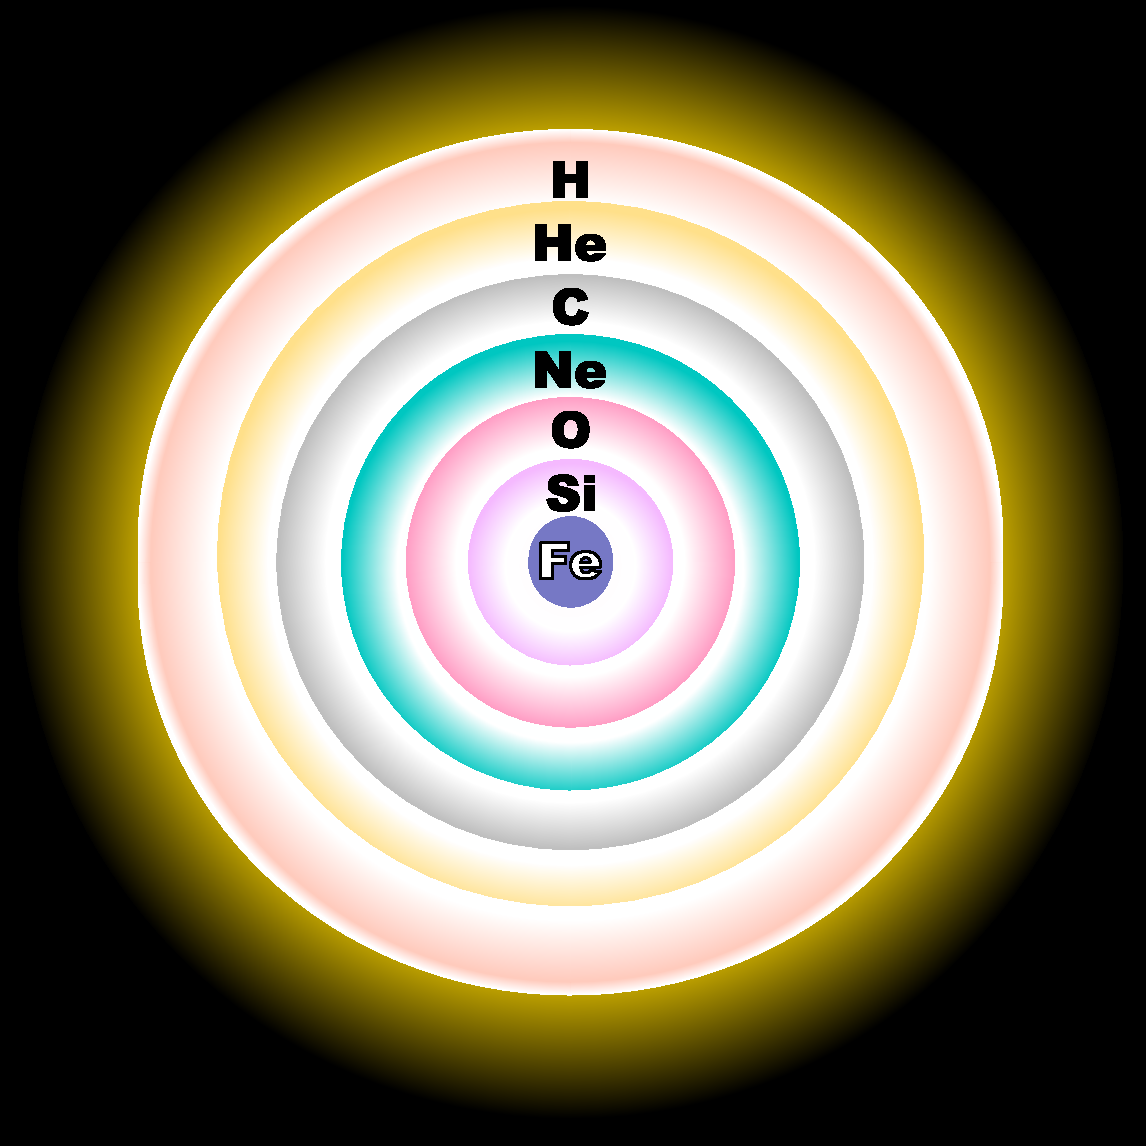
\includegraphics[width=0.7\textwidth]{chapter_intro/plots/fusion_shells.pdf} 
   \caption[Shell Burning of a massive star before SN II]{Shell Burning of a massive star before \glsentryname{snii}. (Source  Wikipedia)}
   \label{fig:fusion_shells}
\end{figure}


In the carbon burning stage, two \nucl{C}{12} nuclei are fused to a highly excited state of \nucl{Mg}{24} magnesium which then decays slowly to via three possible channels (see Equation \ref{eqn:c_burning}) .
\begin{eqnarray}
\nucl{C}{12}+\nucl{C}{12}\rightarrow \nucl{Mg}{24}^{*}&\rightarrow&\nucl{Mg}{23}+\textrm{n} \nonumber \\
	&\rightarrow&\nucl{Ne}{20} + \alpha \nonumber \\
	&\rightarrow&\nucl{Na}{23} + \textrm{p} \nonumber \\
	\label{eqn:c_burning}
\end{eqnarray}

Although oxygen has a lower coulomb barrier, the next nucleus to burn after carbon is neon. This layer is composed of  \nucl{O}{16}, \nucl{Ne}{20} and \nucl{Mg}{24} and burns neon with high-energy photons from the tail of the Planck distribution ($\nucl{Ne}{20}(\gamma,\alpha)\nucl{O}{16}$). 

In the next shell there is a composition of mainly \nucl{O}{23}, \nucl{Mg}{24} and \nucl{Si}{28}. The bulk nucleosynthetic reaction is shown in Equation \ref{eqn:o_burning}. 

\begin{eqnarray}
^{16}O+^{16}O\rightarrow^{28}Si&\rightarrow&^{31}S+n \nonumber \\
	&\rightarrow&\nucl{P}{31} + \textrm{p} \nonumber \\
	&\rightarrow&\nucl{P}{30} + \textrm{d} \nonumber \\
	&\rightarrow&\nucl{Si}{28} + \alpha \nonumber \\
	\label{eqn:o_burning}
\end{eqnarray}

The last shell converts \nucl{Si}{28} to \gls{ige}. The obvious reaction $\nucl{Si}{28}+\nucl{Si}{28}\rightarrow\nucl{Ni}{56}$ does not take place, but is replaced by a very complex network of isotopes that results in \gls{ige} being synthesised.

\subsection{Core collapse}

Before the collapse,  the core consists of iron peak elements (see Figure~\ref{fig:fusion_shells}). Neutrino losses during carbon and oxygen burning decreased the central entropy sufficiently so that the core becomes electron degenerate. Such a degenerate core, which is more massive than the \gls{mchan} (adjusted for Y$_e$, entropy, boundary pressure and other parameters) and with no material capable of being burned, will collapse. 

There are two main instabilities that facilitate the collapse. As the density rises the Fermi-Energy becomes high enough for electrons to capture onto iron-group nuclei. This capture process removes electrons that were providing degeneracy pressure and reduces the structural adiabatic index. In addition, the temperature rises to values where the nuclear statistical equilibrium favours many free $\alpha$-particles. The nuclear binding energy of this  $\alpha$-particle rich state is less and the core does not gain sufficient thermal energy to hinder gravity from advancing the collapse.

The collapse eventually leads to nuclear densities, the hard nuclear potential acts as a stiff spring during the compressive phase. It stores up energy and eventually releases this energy resulting in a \textit{core bounce}.  Recent simulations, however show that the ensuing bounce shock is not sufficient for a \snii\ explosion with the shock loosing energy by photo disintegrating the nuclei it encounters (loosing roughly $10^{51}$~\erg\ per 0.1~\msun).

The energy for a successful explosion is now thought to come from neutrino energy deposition. This reinvigorates the shock and leads eventually to an explosion which ejects the envelope of the massive star \citep{1994ApJ...435..339H}. Several variants of neutrino driven explosion now exist, with the neutrino driven convention leading to a Standing Accretion Shock Instability \citep[SASI;][]{2006ApJ...642..401B}, or acoustic g-mode oscillations \citep{2007ApJ...655..416B} . There is not yet a consensus on how stars more massive than 12~\msun actually explode. Regardless, in most cases for stars < 15~\msun, it is believed that a newly born neutron star is left behind in these explosions. 

 \citet{2002RvMP...74.1015W} provide a very comprehensive review of the theory of evolution and core collapse. In particular they go into more detail describing the scenarios after core-bounce.

\subsection{Pair Instability Supernova}
One alternate explosion scenario is the pair-instability supernova. This scenario is believed to only happen in stars with a helium core of more than 40~\msun. After core helium burning the star starts to contract at an accelerated rate, and enters a regime of temperature and density where the energy goes into electron-positron pair production rather than raising the temperature. This leads to a structural instability in the star (where the adiabatic index drops below \sfrac{4}{3}), leading to collapse. This collapse, if significant densities are reached, will result in oxygen fusion, which eventually halts the implosion and the collapse turns into an explosion. For very high stellar masses, it is believed that oxygen fusion does not provide enough energy to halt the contraction and the star collapses to a black hole.


\subsection{Type II Supernovae}
After the collapse of the core, the supernova goes through three distinct phases. The observables of these stellar cataclysms are the light curve, spectra and for one case (\sn{1987}{A}), even the neutrino wind.

The shock-waves generated by the collapsing core reaching the surface, is the first visible signal from the supernova.  \cite{1992ApJ...393..742E} calculated a duration for the so-called shock breakout of \sn{1987}{A} to 180~s, its  luminosity of $5\times10^{44}$\erg~s$^{-1}$. 
Such a breakout thus far has been observed only once - in the case of the lucky observations of \sn{2008}{D} - a \snibc\ \citep{2008Natur.453..469S}. This star, more compact than \sn{1987}{A}, had a shock breakout of 400~s with a luminosity of $6.1\times10^{43}$\erg~s$^{-1}$.

Secondly Shocks in the ejecta and the decay of \Ni\ irradiate the expanding hydrogen envelope and the energy slowly diffuses out causing a plateau, for the \sneiip. \sniil\ have lost most of their extensive hydrogen envelopes and radiate their energy much more quickly - resulting in the observation of a linear decline, rather than a plateau. The last phase begins after the photosphere moves through the entirety of the H envelope, the ejecta transform to become optically thin, the supernova suddenly drops in brightness, and then fades exponentially, following the 77~day half life of \Co, the daughter nucleus of \Ni. Some light might also be produced by shock interaction with the \gls{csm}.

\subsection{Type~Ib/c Supernovae}

In the case of a \snibc, the progenitor has lost at least all of its hydrogen envelope prior to core-collapse. This loss of envelope is presumed to be caused by stellar winds and/or binary interactions \citep{1992ApJ...391..246P}. Thus the hydrogen can not provide a energy buffer and no plateau is visible, similar to a \sniil. Instead the light-curve is powered by radioactive decay after shock breakout, with the energy diffusing out from the core. The missing envelope also causes the lack of hydrogen lines in the spectrum leading to the supernova being classified as Type Ib. If both hydrogen and helium envelopes are lost then the supernova is classified as Type Ic. 
. 


\section{Thermonuclear Supernova Theory}
In this section we will discuss the theory of \sneia\ which are thought to be thermonuclear explosions of degenerate carbon/oxygen matter. The different progenitor scenarios leading to an explosion of a massive white dwarfs are discussed in Section \ref{sec:snia_progenitor}.



\subsection{Progenitors of Type Ia Supernovae}
\label{sec:snia_progenitor}

There are two basic scenarios for \sneia\ progenitors. The \gls{sds} has a white dwarf accreting from a non-degenerate companion until the white dwarf ignites leaving behind the companion star \citep[first introduced by][]{1973ApJ...186.1007W}. In the second scenario,  the \gls{dds}, two white dwarfs merge and ignite, leaving no stellar remnant behind \citep[first suggested by][]{1984ApJ...277..355W,1984ApJS...54..335I}. 

\subsubsection{Single Degenerate Scenario}
The \gls{sds} assumes a binary system with one evolved white dwarf and one non-degenerate companion. In most cases this non-degenerate companion is thought to be a main sequence to red giant star. There are also scenarios that involve `exotic' companions such as helium stars. In most cases, the companion (or \gls{donor}) star is believed to have filled its Roche-Lobe and lose mass via \gls{rlof}.

An outstanding problem of the \gls{sds} is the accretion process.  As most white dwarfs are born with masses significantly less than the \gls{mchan}, they need to accrete mass to reach the critical 1.38~\msun. The accretion process needs to efficiently burn any accreted hydrogen into helium and subsequently to carbon/oxygen to explain its absence in \sneia\ spectra, and to prevent recurrent novae from removing material from the system. Theoretically, there is only a very narrow range of accretion rates that allows the white dwarf to accrete hydrogen, stably burn it and efficiently grow to the \gls{mchan}. \cite{2004A&A...419..623Y} have suggest that rotation of the accreting white dwarfs might increase this very narrow parameter range.

 If the mass-accretion rate is too low, it causes nova explosions which are thought to eject more mass than the accretion prior has gained \citep{Nomoto:1982p451}. However, there are some systems (e.g. \gls{rsoph}, \gls{usco}) that have white dwarf masses close to 1.4~\msun\ which undergo recurrent nova outbursts. It is very likely that these systems were not born with a white dwarf this massive, but that these white dwarfs have successfully grown in mass through the accretion of material. This suggest that in some cases, despite nova outbursts, efficient accretion is possible. Too high accretion rates would cause the binary to be engulfed in an extended red giant envelope. The debris of such an envelope are not seen in most \snia\ explosions - an exception might \sn{2002}{ic}. 
 
There are several possible identified progenitor systems. A class of binaries called \glspl{sss} has a white dwarf accreting hydrogen from a non-degenerate companion at an appropriate rate such that hydrogen and helium burn hydrostatically. In cases where the \gls{wd} is a \gls{cowd}, rather than a \gls{onemgwd}, these objects are strong contenders for SN Ia progenitors \citep[][and references therein]{2006astro.ph..6364D}. Another subclass of possible \gls{sds} progenitors are \gls{amcvn} stars \citep{2005ASPC..330...27N}. In this type of cataclysmic variable, material is accreted onto the \gls{wd} from a helium star or helium \gls{wd} \citep{1992A&A...262...97V}. This scenario would conveniently explain the lack of hydrogen in \snia\ explosions . A \snia\ explosion in such systems is discussed in Section \vref{sec:intro:subchandra}.


\subsubsection{Donor Stars}

The \gls{sds} requires a secondary companion star (also known as donor star). If this companion survives the explosion it would be a calling card for the \gls{sds}. One consequence of this explosion is an unusual spatial velocity of the companion post-explosion. The main fraction of this velocity stems from the gravitational unbinding whereas only a small amount would originate in the kick from the supernova ejecta \citep[see Figure \ref{fig:han2008_vrad};][]{2001ApJ...550L..53C,2008ApJ...677L.109H}. \citet{2000ApJS..128..615M} have simulated the impact of \snia\ ejecta on a main-sequence, sub-giant and red-giant companion. In the case of the main-sequence companion, the supernova ejecta heats a small fraction (1-2\%) of the envelope which is lost post-explosion. \citet{2008A&A...489..943P} have repeated the simulations for the main-sequence companion and find similar results, but suggest that even less mass is lost. Post-explosion the main-sequence star should be very luminous (500 -- 5000 \lsun) and is expected to cool down over next 1000 -- 10,000 years and follow the main-sequence track  \citep{2000ApJS..128..615M}. 

\begin{figure}[tb] %  figure placement: here, top, bottom, or page
   \centering
   \includegraphics[width=\textwidth, trim=0 0 2cm 0, clip]{chapter_intro/plots/theo_vrad.pdf} 
   \caption[Expected escape velocities for donor stars]{Expected escape velocity for different evolutionary states of the donor star based on binary population synthesis \citep[][data kindly provided by Z. Han]{2008ApJ...677L.109H} }
   \label{fig:han2008_vrad}
\end{figure}

For the sub-giant companion the simulations show very similar results to the main-sequence companion. The sub giant looses only a small fraction of the envelope (10 -- 15\%) and like the main-sequence star, it will be very luminous shortly after the explosion. After thermal equilibrium is established, the companion will return to a post-main-sequence track. 

The case of the red-giant, however, is different. \citet{2000ApJS..128..615M} suggest that it will lose most of its loosely bound envelope. Post-explosion core contracts and the temperature rises to more than $3 \times 10^4$~K. The object may appear as an under luminous main-sequence O or B star. \cite{2009A&A...493.1081J} have suggested the population of low-mass single white dwarfs to be the remaining cores of such red-giant donor stars. This would result in a convenient explanation for the existence of these objects. 

One feature of surviving companions may be an unusually large rotational velocity post-explosion \citep[][Chapter \ref{chap:sn1572_starg} of this work]{2009ApJ...701.1665K}. Due to tidal coupling during the \gls{rlof} phase, the rotational velocity  of the donor star, post explosion, is directly tied to the binary rotational velocity (see Figure \ref{fig:han2008_vrot}). Since stars of F spectral-type and later do not display such high rotational velocities, this feature is a very useful discriminant when looking for donor stars. 

\begin{figure}[tb] %  figure placement: here, top, bottom, or page
   \centering
   \includegraphics[width=\textwidth, trim=0 0 2cm 0, clip]{chapter_intro/plots/theo_vrot.pdf} 
   \caption[Expected rotational velocities of donor stars]{Expected rotational velocity for different evolutionary states of the \glsentryname{donor} star post-explosion based on binary population synthesis \citep[][data kindly provided by Z. Han]{2008ApJ...677L.109H} }
   \label{fig:han2008_vrot}
\end{figure}


There have been several attempts to find these objects in ancient supernova remnants. \citet{1980ApJ...241.1039S} found a OB subdwarf star located 2.5\arcmin\ from the centre of the remnant of \sn{1006}{} and suggested this as the donor star. Subsequent analysis by \cite{1997ApJ...477L..53W, 1983ApJ...269L...5W} however, have revealed strong \ion{Fe}{2} features with a profile broadened by a few thousand \kms and ionised redshifted silicon features. In the very likely case that these features are caused by the remnant this indicates the star to be located behind the remnant rather than being involved in the \snia\ explosion as a donor star.
 
The search for donor stars in ancient remnants is one of the main parts of this thesis and we direct the reader to Chapter \ref{chap:sn1572_starg} through Chapter \ref{chap:sn1006}.



\subsubsection{Double Degenerate Scenario}
\citet{1984ApJ...277..355W} and \citet{1984ApJS...54..335I} were the first to suggest merging white dwarfs as progenitors for \snia. There are several advantages to the \gls{dds}. For example, it naturally explains the lack of hydrogen in \snia\ spectra. The accretion problem encountered in the \gls{sds} is dispensed with in the \gls{dds}, as long as the sum of masses of both \gls{cowd}'s is above \gls{mchan} - although new ideas might make this an upper limit rather than a requirement \citep{2010ApJ...722L.157V}. 

One problem with this scenario, however, is that most \snia\ form a relatively homogeneous class. It is hard to reconcile this fact with the merger of two white dwarfs with different initial masses, composition, angular momenta and different impact parameters. A potentially even larger problem, however, is that the accretion of the disrupted lighter white dwarf onto the more massive white dwarf is thought to lead to \gls{aic} rather than a thermonuclear explosion (see Section \ref{sec:white_dwarfs}).

\cite{2010Natur.463...61P} have simulated the merger of two equal-mass white dwarfs (0.9~\msun) and conclude that the outcomes of these mergers might be subluminous \sneia.

In summary, mergers of white dwarfs might be able to explain some of the \snia\ class. It is however still debated if these events are responsible for the abundance \gls{branchnormal} \sneia. 

\subsection{Evolution and Explosion of Type Ia Supernovae}

\subsubsection{White Dwarfs}
\label{sec:white_dwarfs}
\glspl{cowd} are thought to be the progenitor stars of \sneia. White dwarfs are among the most common stellar objects that are not composed primarily of hydrogen, which is consistent with the lack of hydrogen in \snia\ spectra. Furthermore, there is a clear theoretical avenue to exploding white dwarf stars, through accretion of material to near the \gls{mchan}. It is general believed that these objects accrete matter (for the possible scenarios see section \ref{sec:snia_progenitor}) until they get close to the \gls{mchan}. It is a delicate balance between conditions for ignition that results in a thermonuclear run-away and reaching the \gls{mchan} threshold, which would lead the collapse of the star to a neutron star.
 
There are three main classes of white dwarfs: helium \glspl{wd}, \glspl{cowd} and \glspl{onemgwd}. Originally \glspl{onemgwd} were called ONeMg WDs but the mass fraction of magnesium had been overestimated and thus now only oxygen and neon are mentioned \citep{1996ApJ...460..489R}. 

The accretion onto a helium \gls{wd} would lead to helium burning well before the \gls{mchan} and thus these objects are not considered as potential progenitors. Although not considered as the \snia\ progenitor itself helium, \glspl{wd} as companions to \glspl{cowd} are an interesting suggestion as \snia\ progenitor systems (see Section~\ref{sec:intro:subchandra}). The ultimate fate of an accreting \gls{onemgwd} is thought to be the collapse into a neutron star. Theoretical models predict that before oxygen can be ignited, electron capture begins in the core ($\Ne(e^-,\nu)\F[20](e^-,\nu)\Ox[20]$). Heating by the resulting $\gamma$-rays starts explosive oxygen burning. However, the electron-capture is much faster than the oxygen burning and promotes the collapse to a neutron star \citep{1991ApJ...367L..19N, 2005A&A...435..231G}. 

The favoured progenitor for a \snia\  are \glspl{cowd}. Theoretical calculations predict that these objects ignite when very close to the \gls{mchan} (1.38~\msun). The vast majority of white dwarfs are born with masses around 0.6~\msun\ \citep{2007MNRAS.375.1315K} due to the large abundance of  $\approx 1~\msun$ stars compared to stars with a mass $> 5~\msun$ which would turn into more massive \glspl{wd}.  It is, however, quite frequent to have \gls{wd} stars built up to more than 1~\msun\ through mass transfer in binary systems with an intermediate mass companion ($ 2~\msun < M < 8~\msun$) . Such systems are thought to be the eventual progenitors of \snia.

\subsubsection{Pre-Supernova Evolution}
The white dwarf gradually accretes more and more material. Close to \gls{mchan} mild carbon burning ensues
\begin{align}
\nonumber
\Carb(\Carb,p) &\rightarrow \Na \\  \nonumber
\Carb(\Carb,\alpha) &\rightarrow \Ne \\ 
\Carb(\Carb,n) &\rightarrow \Mg[23],
\end{align}
but is mediated by photon and neutrino losses \citep{2005NuPhA.758..463L, 2007nps..book.....I}. As these cooling processes become less effective convection starts in the core and the energy output in the core increases. At this stage the thermal structure is largely controlled by what is termed \gls{urca} pairs. These reaction pairs consist of alternating electron captures and $\beta^-$~decays involving the same pair of parent and daughter nuclei. Two prominent examples which are important in pre-supernova evolution are \Ne[21]/\F[21]:
\begin{align}
\nonumber
\Ne[21](e^-, \nu) &\rightarrow \F[21] \\
\F[21](\beta^- \nu) &\rightarrow \Ne[21]
\end{align}
These processes can lead to either cooling or heating \citep{2005NuPhA.758..463L}.

At present, the pre-supernova evolution has proven difficult to model theoretically as it is likely to be non-local, time-dependent, three-dimensional and stretches over hundreds of years. The exact conditions at the time of explosion are therefore poorly constrained, and all explosion models have to assume simple initial conditions. The main steps leading to the explosion follow.

\subsubsection{Explosion mechanisms}

\paragraph{Ignition} The \gls{urca} processes will dominate core evolution for the last thousand years until explosion. As the temperature rises to $T\approx7 \times 10^8$~K \citep{2000ARA&A..38..191H} the convection time ($\tau_c$) increases and becomes comparable to the burning time ($\tau_b$). Consequently the convective plumes burn as they circulate. Once the temperature reaches $T\approx 10^9$~K, $\tau_b$ becomes very small compared to $\tau_c$ and carbon and oxygen largely burn in place. This is the moment of ignition. As the convective plumes burn while they rise it is likely that the initial flame seed does not start in the centre of the core. \cite{2005A&A...431..635R} have used multiple flame seeds in their three dimensional full star models.

\paragraph{Thermonuclear Explosion} After ignition, there has historically been two main options. The first option was the complete detonation (supersonic flame front) of the \gls{cowd}\ \citep{1969Ap&SS...5..180A}. It was quickly, discovered, however that this method burns the entire star to \gls{nse} (\Ni\ dominant),  and thus leaves none of the \glspl{ime} observed in \sneia. 

To counteract this problem, it was suspected that the star instead of detonating would deflagrate (subsonic flame wave, mediated by thermal conduction). The fuel in front of the deflagration becomes rarefied by the energy from the flame, with hot light burning bubbles rising into the cold dense fuel creating Rayleigh-Taylor instabilities (see Figure \ref{fig:snia_ddt_roepke2007} at t=0.72~s). 
Detailed calculations show that once the deflagration wave has run through the star, the resulting production of \Ni[56] is lower than that observed in \sneia. More critically \glspl{ime} are left throughout the expanding debris, leading to an un-observed distribution of \glspl{ime} at low velocities \citep{2007Sci...315..825M}.

The currently favoured scenario is the one of delayed detonation. Here, the star initially burns like in the deflagration scenario with the inhomogeneities in the deflagration front producing hot spots. We refer the reader to \citet{2010ApJ...710.1683S} and references therein, for a detailed explanation of the transition from a deflagration to a detonation wave. Once the detonation wave has formed it travels through the unburned star - not penetrating the already deflagrated nuclear ashes. This produces an event which observationally is a good match to the spectral evolution of \sneia\ \citep[e.g.][]{2009Natur.460..869K}. Figure \ref{fig:snia_ddt_roepke2007} shows clearly how the detonation wave wraps around the cold ashes over the course of the detonation. An open question is if and how these transitions from deflagration to detonation occur in \sneia.


\begin{figure}[tb] %  figure placement: here, top, bottom, or page
   \centering
   \includegraphics[width=1\textwidth]{chapter_intro/plots/ddt_roepke08.pdf}
   \caption[Delayed detonation simulation from \citet{2008NJPh...10l5009R}]{Delayed detonation simulation from \citet{2008NJPh...10l5009R}. The upper panels show the deflagrated interior (marked in blue) and the detonation ignition point (small white sphere). The detonation wave wraps around the deflagration ash and consumes the cold fuel. (Image reproduced with kind permission of Fritz R\"{o}pke)}
   \label{fig:snia_ddt_roepke2007}
\end{figure}


\paragraph{Sub Chandrasekhar Mass detonations}
\label{sec:intro:subchandra}
\cite{1990ApJ...354L..53L}, \citet{1992ApJ...386L..13S}, \citet{1995ApJ...452...62L} and \citet{2010ApJ...714L..52S} have explored the detonation of \glspl{cowd} at sub \glspl{mchan}. \citet{2010ApJ...714L..52S} show that the detonation of a sub \gls{mchan} \gls{cowd} reproduce observed light-curves and early-time spectra of \sneia\ fairly well.

A significant issue in this scenario is the ignition. \cite{2010A&A...514A..53F} have studied an explosion mechanism in which a surface detonation of a helium shell drives a shock-wave into the core. In the core this shock wave triggers an ignition by compression.  As an initial model they use a \gls{cowd} accreting from a helium rich companion building a thin helium shell around its CO interior \citep[described in][]{2007ApJ...662L..95B}. This helium shell is ignited and sends out a shock wave. As the helium flame spreads in the shell around the star it sends a shock wave into the core. Once the shock waves converge off-centre they create an environment hot and dense enough that the ignition of a detonation wave may be possible (see Figure \ref{fig:subch_fink2010}.) 

This scenario reproduces the intrinsic luminosity variability in the class of \snia\ as each exploding white dwarf can have a different mass, but might predict too much variation. 

\begin{figure}[tb] %  figure placement: here, top, bottom, or page
   \centering
   \includegraphics[width=\textwidth]{chapter_intro/plots/fink2010.pdf} 
   \caption[Helium shell ignition leading to sub \glsentryname{mchan} detonation]{The ignition point of the helium shell is marked in the upper left image. We can follow the helium shell sending shock waves into the core of the white dwarf. They converge in the lower left image at the opposite site of the Carbon/Oxygen core \citep[data from][Figure kindly provided by Michael Fink]{2010A&A...514A..53F}. }
   \label{fig:subch_fink2010}
\end{figure}

\paragraph{Super Chandrasekhar Mass Detonations}
As well as sub \gls{mchan} explosions, the community has also studied the explosion of white dwarfs with $M>\glssymbol{mchan}$. There have been a small number of \sneia\ which were extremely luminous (e.g. \sn{2003}{fg}, \sn{2006}{gz}, \sn{2007}{if} and \sn{2009}{dc}) suggesting ejecta masses of much more than 1.4~\msun \citep{2006Natur.443..308H,2007ApJ...669L..17H,2009ApJ...707L.118Y,2010ApJ...713.1073S,2010ApJ...714.1209T,2011MNRAS.410..585S,2011MNRAS.412.2735T}. This raises the question why these objects do not undergo \gls{aic}. \cite{2005A&A...435..967Y} suggest that through rapid rotation these objects will increase the effective \gls{mchan}. Another possibility is the merger of two massive white dwarfs. \citet{2010Natur.463...61P} however suggested, for the merging of equal-mass 0.9~\msun\ \glspl{cowd} (a total mass of 1.8~\msun), the resulting supernova would resemble the class of \gls{91bg} objects. A core collapse scenario for some of these events has also been constructed. The number of observed super \gls{mchan} supernovae is as of yet too low to define common characteristics or a class.


\subsection{Constrains for different progenitor scenarios}
\label{sec:progenitor_constraints}
The question of the progenitors of \sneia\ is a main part of this thesis and one of the most highly debated subjected in current \sneia\ research. There are various arguments for and against the \gls{sds} and the \gls{dds}, with some suggesting that both scenarios contribute to the class of \gls{branchnormal} \sneia.


\cite{2007Sci...317..924P} have found a variable blue-shifted sodium absorption feature using high-resolution spectra of \sneia. This suggests that there is sodium rich material in the line-of-sight. The variability suggests that this material is close to the supernova explosion. One explanation of this variability is the change in the ionisation state of the sodium atoms in a nearby \gls{csm} caused by the variable \snia\ radiation field. Very recently a study by \cite{2011arXiv1108.3664S} observed sodium features in 30 \sneia. They found that many of these \sneia\ show blue-shifted sodium features relative to the host galaxies rest frame, which can be explained by expanding winds from the progenitor system. Finally, \citet{2011A&A...530A..63P} have seen similar features in the recurrent nova \gls{rsoph}. This could hint that recurrent novae with red giant donor stars might be responsible for some \sneia. 

\cite{2010ApJ...719..474D} have not found enough \gls{sss} to account for the rate of \sneia. In addition, \cite{2010Natur.463..924G} have not found enough accumulated X-ray flux from elliptical galaxies if all \snia~progenitors were \gls{sss}\ (assuming the X-Ray flux calculated for these objects is correct). The main caveats here are that the \snia-progenitors might only be in the \gls{sss} phase for a short amount of time and at other times, these objects could be engulfed in a envelope, which would reprocess the produced \xray s to optical or infrared wavelengths. In stark contrast to the negative \xray~studies described above, \citet{2008Natur.451..802V} have suggested that they found the progenitor of the Type Ia \sn{2007}{on} in \xray s. Further analysis has put this claim in doubt \citep{2008MNRAS.391..290R}. Although the detection might have been spurious, their technique remains promising: Following up \sneia\ in \xray-archives could detect potential \sneia\ progenitors in a pre-explosion \xray\ phase and could confirm the \gls{sss}~scenario for some \sneia.

It remains a mystery that \sneia\ do not show lines of hydrogen which might be expected from the wind or stripped envelope in the \gls{sds}. \citet{2007ApJ...670.1275L} have searched in the nebular spectra of two \sneia\ for hydrogen and place an upper limit of 0.1~\msun\ for both these explosions. On the other hand, \citet{2011ApJ...730L..34J} suggest that a red giant donor could significantly shrink during the \gls{rlof} and the material stripped by the ejecta might be negligible. This would place the the stripped hydrogen below the current detection limit. 

\cite{2010ApJ...708.1025K} predicts excess in \gls*{uv} flux in the \snia\ light curve at early times for \snia\ from single degenerate systems. This effect depends on orientation of the system to the line of sight and the state of the donor. The effect would be biggest for a red giant donor star. \cite{2010ApJ...722.1691H} do not see this excess in the \gls{sdss} supernova set indicating that the red giant channel is not common for \sneia. A study by \cite{2011arXiv1106.4008B} using the \gls{snls} data set comes to the same conclusion. To conclusively state a lack of this predicted excess a big sample of very early light curves is needed, which does not exist yet.

Radio observations in the case of \sneia\ can, for example, reveal the shock interaction of the ejecta with the \gls{csm}. The \gls{sds} predicts a more dense \gls{csm} than the double degenerate scenario. \citet{2011arXiv1105.6188H} have stacked radio observations of \sneia\ in the visibility plane and have not detected any source. At present, it is not clear that this limit is in conflict with the \gls{sds}. Future stacked \gls{evla} measurements will push the limits substantially down and will hopefully provide constraints that will allow us to rule out one or the other scenario, at least for some \sneia.


Finding a donor star of the \gls{sds} in a \gls{snr} post-explosion would resolve the question for the progenitor system, at least in the searched remnants. The main work of this thesis investigates this technique and we will refer the reader to Chapter \ref{chap:sn1572_starg} through \ref{chap:sn1006}. 

Population synthesis together with observations of \glspl{dtd} are an important step in exploring the different progenitor scenarios. \citet{2008ApJ...683L.127H, Han:2004p444}  have explored the \gls{sds} parameter space and suggest, when compared to observations, that the \gls{sds} can almost explain the observed \gls{dtd} (for references on \dtd\ see section \ref{sec:sn_rates}). \citet{2009ApJ...699.2026R} and \citet{2010A&A...515A..89M}, however, have explored the \snia-rate using several progenitor scenarios (\gls{sds}, \gls{dds} and \gls{amcvn}). Both suggest that the \gls{sds} on its own can not explain the observed \sneia\ rate. The rate of the \gls{dds} seems to be much closer to the observed frequency. Possibly a mix of all channels is required to explain the observed rate. 


In addition to the standard SD and DD channels, alternative scenarios are continually being explored. For example, a \emph{core-degenerate} scenario in which a white dwarf merges with the hot core of a massive \gls{agb} star \citep{2011arXiv1106.2027I}. Another alternative is given by \citet{2011arXiv1102.4342D} and \citet{2011ApJ...730L..34J}, who suggest that the accreting white dwarf would be spun-up during accretion. The ignition of these highly spinning white dwarfs would be delayed and the companion might have time to evolve  substantially from its \gls{rlof} phase. 

\citet{2010ApJ...722L.157V} explores the merger of two equal mass white dwarfs with a total mass less than the \gls{mchan}. When coupled with the work on sub-Chandrasekhar mass detonations by \citet{2010ApJ...714L..52S}, this might actually provide a viable progenitor scenario. Its main advantage is the predicted rate of these low-mass white dwarf mergers might be high enough to reproduce the observations, but it is yet unclear if the conditions for an ignition can be reached in such a merger. 

In summary, the question of the progenitors of \sneia\ remains one of the most highly debated topics in \sneia\ research. We have not yet found a scenario that elegantly explains all aspects of the \snia\ phenomenon. In addition, different measurements seem to provide conflicting evidence for either scenario. More extensive and novel observations of \sneia\ and \gls{snr} will hopefully identify the nature of \snia\ progenitors scenario.



\section{Thesis motivation}
One of the pivotal moments in astronomy in recent years was the discovery of the accelerating expansion of the universe by \citet{1998AJ....116.1009R} and \citet{1999ApJ...517..565P}. This discovery made \sneia\ the cynosure of the astronomical community. There have been many advances in recent years in the understanding of these cataclysmic events (explosion models, rates, etc.). One critical piece of the puzzle, however, has so far eluded discovery: the progenitors of \sneia. This work's main aim is to look for evidence for one \snia\ progenitor scenario. The \gls{sds} proposes a white dwarf accreting from a non-degenerate donor star. All calculations suggest that this donor star will survive the explosion and would be visible thereafter. We have tried to find this companion in two of the three easily accessible ancient supernova remnants (\sn{1572}{}\ and \sn{1006}{}). In Chapter~\ref{chap:sn1572_starg} we have obtained spectra of \starg, which had been suggested as the donor star of SN1572 \citep{2004Natur.431.1069R}. Although we confirmed some of the suggested parameters, we could not reproduce the unusually high radial velocity, which led to the claim.  We also showed that the star exhibited no rotation, at odds with the star being the donor star.

We revisited \sn{1572}{}\ in Chapter \ref{chap:sn1572_hires} with new observations of \starg\ and five other stars in the neighbourhood of \sn{1572}{}. This work indicates \starg\ is consistent with a background interloper, and is likely not to be the donor star (although it is hard to completely rule any star out). We discovered a curious A-star located right in the centre of SN1572. Despite its a priori unusual parameters, we are unable to reconcile this star (\starb) with any feasible progenitor model. 

\sn{1006}{} provides an additional opportunity to search for progenitor stars. It is the closest known remnant of a \snia\ (2~\kpc) and is largely unreddened. We have obtained 80 spectra of stars close to the centre of the remnant and present them in Chapter \ref{chap:sn1006}. Again we do not find any obvious donor stars. We have obtained spectra of stars around \sn{1604}{} but these are not presented in this thesis. They will be analysed as part of future work.

Progenitor hunts provide us with information of the scenarios pre-explosion. Spectra, on the other hand, help to unravel the physics during and post-explosion. \cite{2008MNRAS.386.1897M} have developed a code that can produce synthetic \snia\ spectra from fundamental input parameters. Fitting an observed \snia\ is, for the moment, a manual task. This requires many days, if not weeks, of tweaking. The deluge of spectroscopically well-sampled \sneia\ from surveys is already upon us. Manual analysis of all of these spectra is impossible. The information about the explosion hidden in the spectra is, however, crucial to our understanding of these events. In Chapter \ref{chap:dalek} we present our work towards automating this fitting process. We have tried a variety of algorithms to explore the vast and extremely complex search space. Working together with members of the computer science community, we are exploring the use of genetic algorithms to solve this problem. This thesis does not attempt to completely solve this problem, but we present preliminary methods in \snia-fitting in Chapter \ref{chap:dalek}. When completed, we can apply this method not only to fitting \snia, but fitting different supernovae and to other areas of astronomy. 

In summary, this work explores two areas of supernova physics: progenitors and explosion physics. The hunt for progenitors has not yielded obvious candidates, but may suggest a rethinking of the `normal' \gls{sds}. The automated fitting of supernova spectra is in a preliminary stage. We have, however, shown that it is possible to explore the parameter space in an automated fashion. This will hopefully yield elemental abundances and energies for many thousands of supernovae. The close collaboration with computer science community was very helpful and shows how important cross-disciplinary research is in the modern era of science. 


